\documentclass[10pt,letterpaper]{article}
\renewcommand\familydefault{\sfdefault}

\usepackage{amsmath}

\usepackage[T1]{fontenc} 
\usepackage[utf8x]{inputenc}
\usepackage[british]{babel}
\usepackage{graphicx}% Include figure files
\usepackage{blindtext} 

\usepackage{fancyvrb,xcolor}
\usepackage{upquote,textcomp}

%%% Margins
\oddsidemargin=-0.50cm
\textwidth=17.0cm
\topmargin=-2.54cm
\headheight=0cm
\headsep=2cm
\textheight=23.8cm


\usepackage{hyperref} % for urls


% Default fixed font does not support bold face
\DeclareFixedFont{\ttb}{T1}{txtt}{bx}{n}{8} % for bold
\DeclareFixedFont{\ttm}{T1}{txtt}{m}{n}{8}  % for normal

% Custom colors
\usepackage{color}
\definecolor{deepblue}{rgb}{0,0,0.5}
\definecolor{deepred}{rgb}{0.6,0,0}
\definecolor{deepgreen}{rgb}{0,0.5,0}
\definecolor{deepgray}{rgb}{0.5,0.5,0.5}

\usepackage{listings}

\lstdefinestyle{myCustomPythonStyle}{
	language=Python,
	basicstyle=\linespread{1}\small,
	otherkeywords={self},             % Add keywords here
	keywordstyle=\ttb\color{deepblue},
	emph={MyClass,__init__},          % Custom highlighting
	emphstyle=\ttm\color{deepred},    % Custom highlighting style
	commentstyle=\ttm\color{deepgray},
	stringstyle=\color{deepgreen},
	frame=tb,                         % Any extra options here
	showstringspaces=false,
	columns=fullflexible,
	keepspaces=true,
	literate={-}{-}1,				% To avoid problems with hyphen -
}


\usepackage{dirtree}



\makeatletter 
  \renewcommand\verbatim@font{\normalfont\ttfamily\color{blue}}
\makeatother

\parindent=0mm 			% Remove french indent
\setlength{\parskip}{0.3cm}


\title{ScientoPy - User Manual}


\begin{document}



\begin{center}
{\LARGE \textbf{ScientoPy v 3.2.0, Installation and User Manual\\}}
\vspace*{0.5cm}

\includegraphics[scale=0.2]{./figures/escudoUnicacuaSolo.eps}\\
\vspace*{0.5cm}
Juan Pablo Ruiz Rosero\\
\texttt{jpabloruiz@unicauca.edu.co} \\
\end{center}

\tableofcontents

\newpage

\section{Installation}

\textbf{Requirements:} Python 3.9 or higher.

\begin{enumerate}
\item For Windows download and install Python 3 (version 3.9 or higher) from: \\ \url{https://www.python.org/downloads/}.
\item For Debian or Ubuntu run this command to install Python3 and tkinter:
\begin{verbatim}
sudo apt-get install python3 python3-tk python3-pip python3-pil python3-pil.imagetk
\end{verbatim}

\item Clone the repository:
\begin{verbatim}
git clone https://github.com/jpruiz84/ScientoPy
\end{verbatim}

\item Create a virtual environment and install dependencies:
\begin{verbatim}
python3 -m venv venv
source venv/bin/activate        # Linux/macOS
# venv\Scripts\activate          # Windows

pip install --upgrade pip
pip install -r requirements.txt
\end{verbatim}

\end{enumerate}

\section{Download the bibliometric dataset}
This section describes how to download the proper dataset from Scopus and WoS. Define a search criteria that will be used for Scopus and WoS. For this guide and for the example dataset we are using: "Bluetooth low energy"

\subsection{Download the dataset from Scopus}
\begin{enumerate}
\item Make your search with the defined search criteria for Article title, Abstract, Keywords. 
\item Select all the results and click on Export:
	\begin{center}
		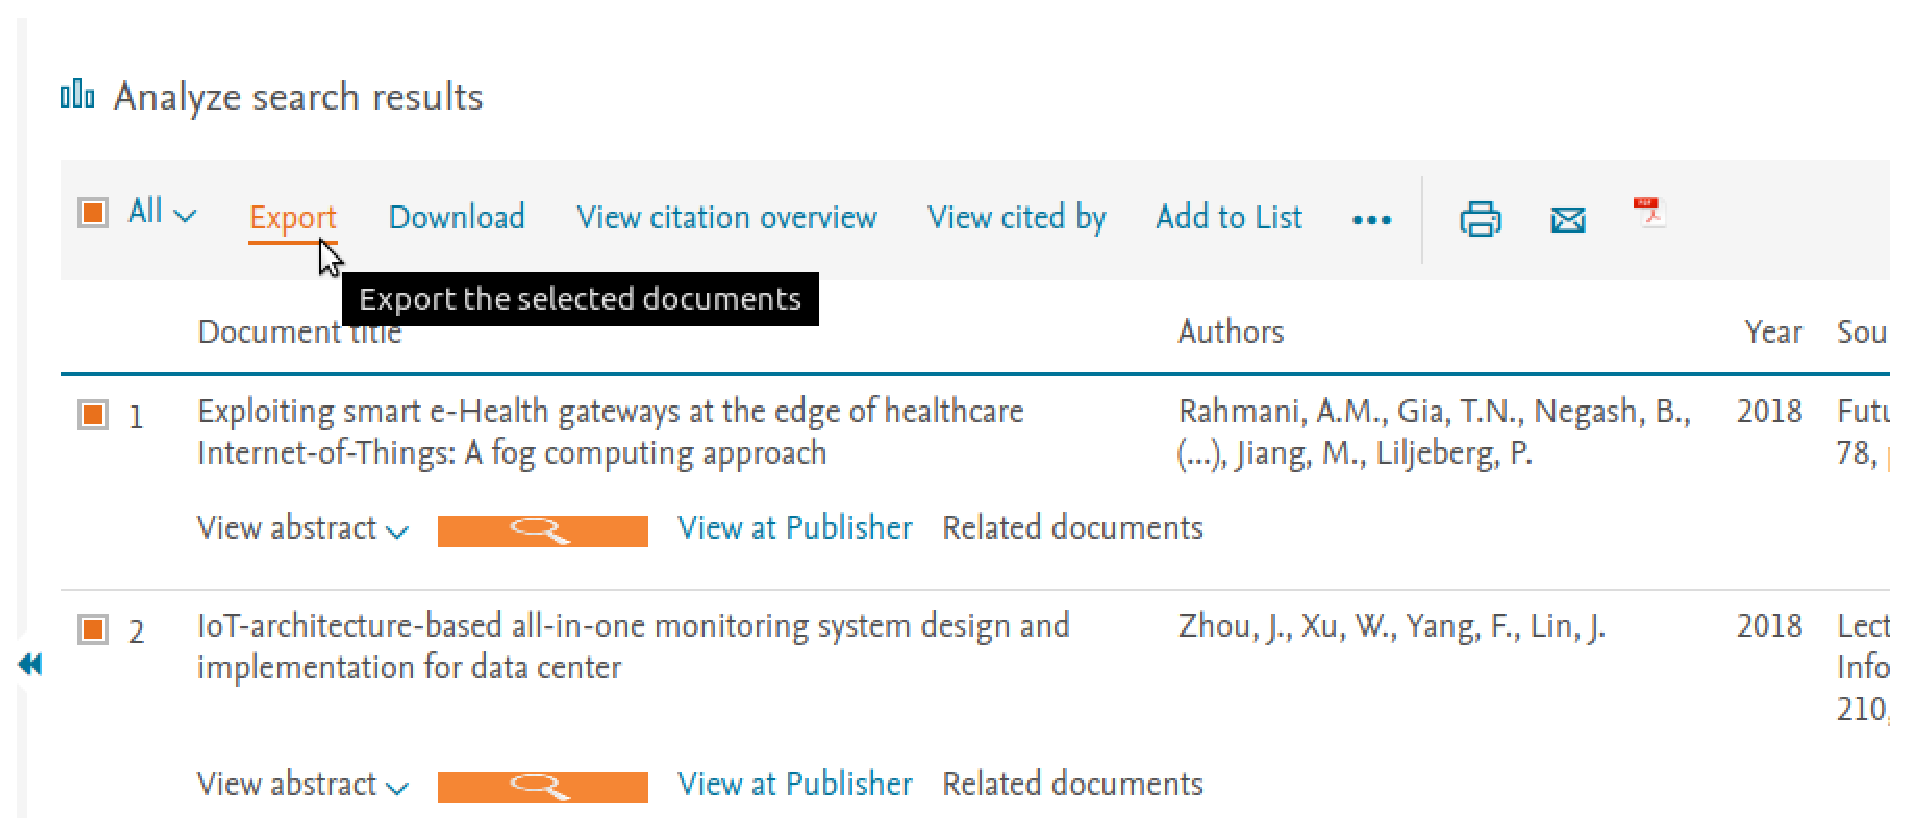
\includegraphics[scale=0.33]{./figures/scopus1.eps}
	\end{center}

\item Select as method of export \textbf{CSV (Excel)}, and select the Customize export \textbf{Citation information, Bibliographical information, Abstract and Keywords}, then click on Export: 
	\begin{center}
		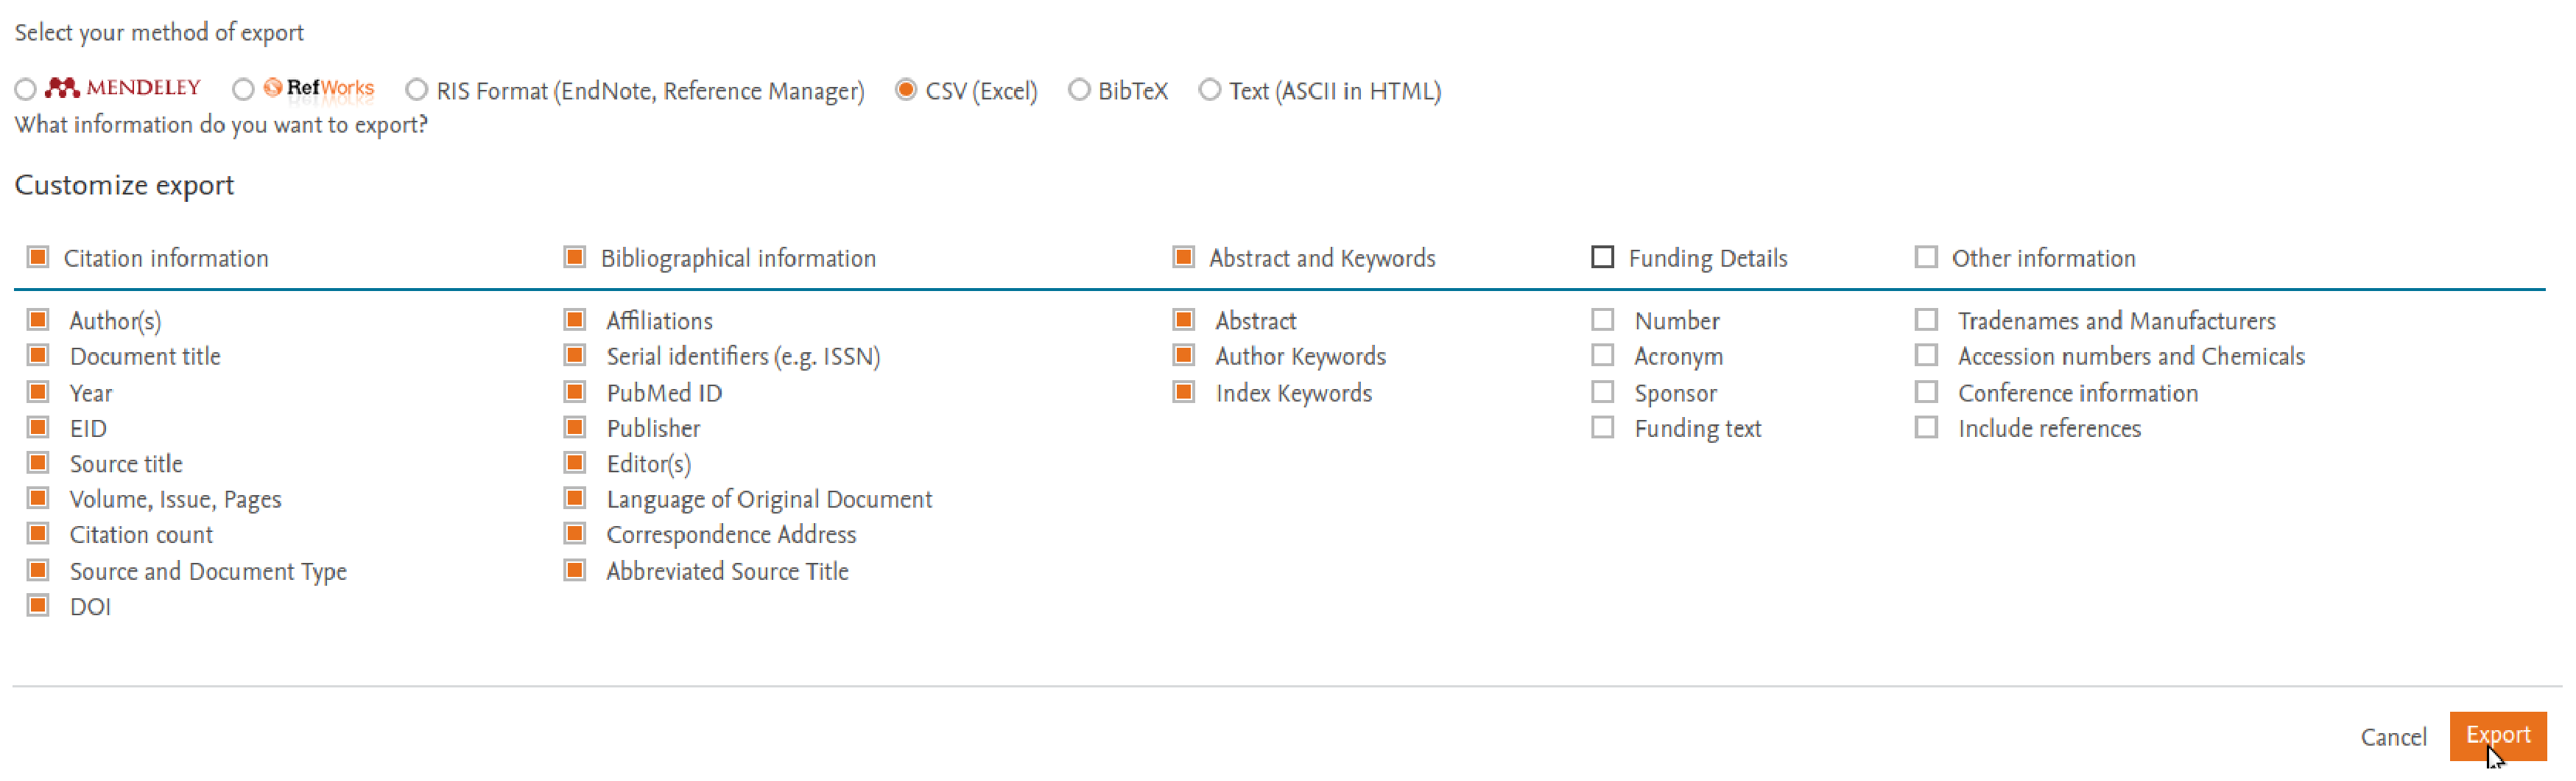
\includegraphics[scale=0.3]{./figures/scopus2.eps}
	\end{center}

\item Save the file on the folder \verb|/ScientoPy/dataIn|
\end{enumerate}


\subsection{Download the dataset from WoS}
\begin{enumerate}
\item Make your search with the defined search criteria for Topic. 
\item Select \textbf{Save in Other File Formats}
	\begin{center}
		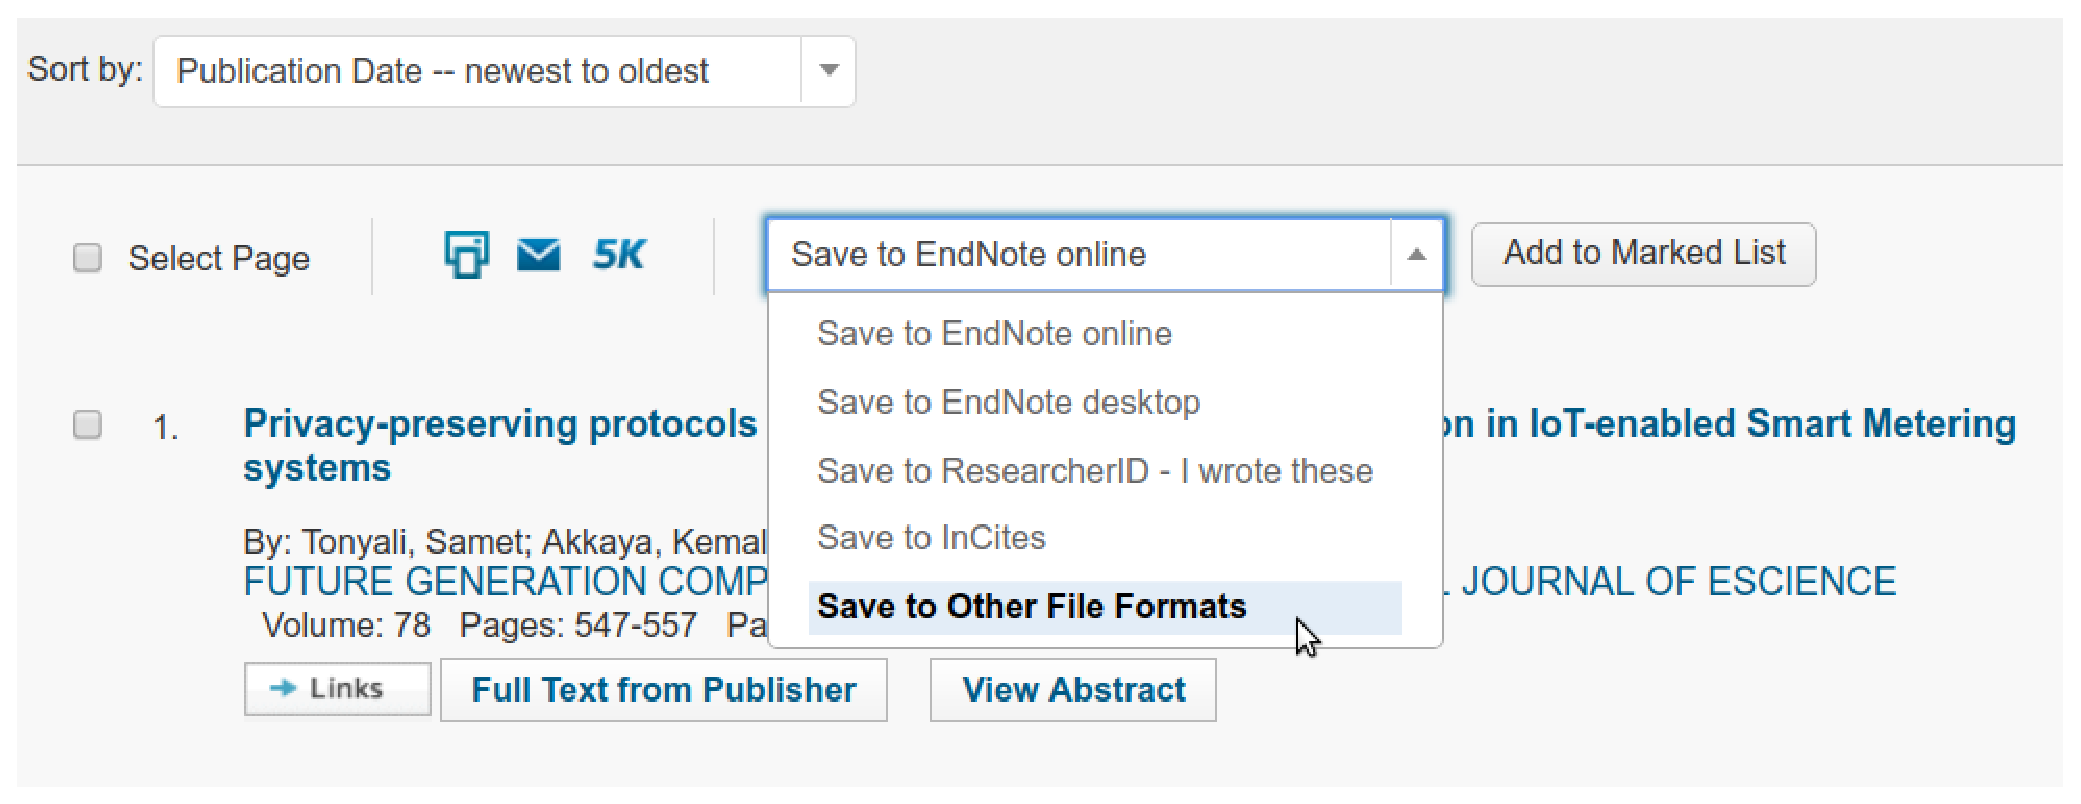
\includegraphics[scale=0.33]{./figures/wos1.eps}
	\end{center}

\item Select the number of records to download, on Record Contented select \textbf{Full Record and Cited References}, on File Format select \textbf{Tab-delimited (Win, UTF-8)}, and click on Send.
	\begin{center}
		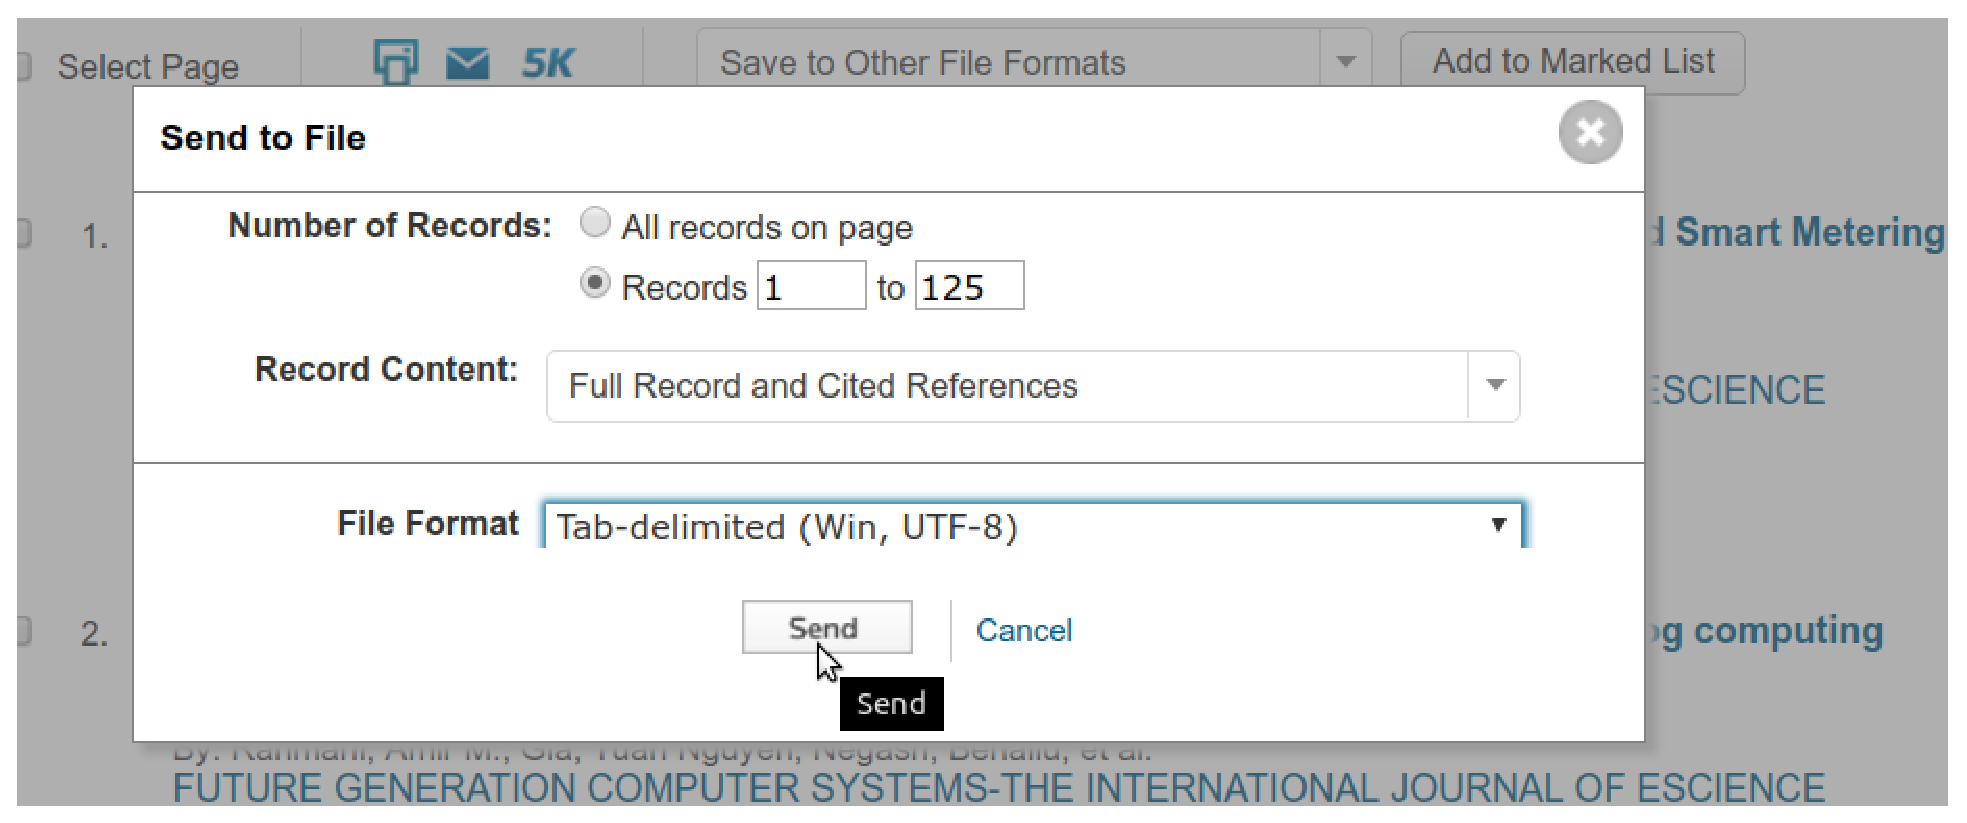
\includegraphics[scale=0.33]{./figures/wos2.eps}
	\end{center}

\item Save the file on the folder \verb|/ScientoPy/dataIn|
\end{enumerate}

\section{Running the ScientoPy scripts}

This section describes the ScientoPy scripts to preprocess and analyze the bibliometric dataset. 

\subsection{Preprocessing}

First we need to preprocess the downloaded dataset. The preprocessing improves the dataset readability and precision through the following steps:

\begin{enumerate}
\item \textbf{Document type filtering:} By default, ScientoPy filters publications classified as: Conference Paper, Article, Review, Proceedings Paper, or Article in Press. Other document types (book chapters, short surveys, letters, notes, editorials, erratum, reports, etc.) are excluded.

\item \textbf{Field tags correlation:} WoS and Scopus use different field tags for their datasets. ScientoPy converts WoS two-character field tags to Scopus style fields and uses the Scopus format internally.

\item \textbf{Author's name normalization:} To ensure consistency between WoS and Scopus author name formats, ScientoPy applies the following normalizations:
\begin{itemize}
\item Replace Scopus dot and comma separators with semicolons
\item Remove dots and commas from WoS and Scopus author fields
\item Remove accents marks and special characters
\item Convert the first author last name to upper case
\end{itemize}

\item \textbf{Duplicated removal:} ScientoPy detects duplicated documents based on the DOI, the normalized title, and the normalized first author last name. When duplicates are found between WoS and Scopus, ScientoPy keeps the WoS document and removes the Scopus one. For duplicated documents with different ``cited by'' counts, ScientoPy calculates the average times cited between the two entries and assigns it to the kept document.

\item \textbf{Times cited:} When a document is duplicated, the \textit{times cited} field often does not match between databases. ScientoPy gets the average times cited between the two duplicated documents and sets it in the document that is going to be kept. This value is used later for h-index calculations.

\item \textbf{Country and institution extraction:} ScientoPy extracts the document's country from all author's affiliations (last section after the comma). Institution names are extracted from the first section before the comma in WoS documents' affiliation fields. Country names are normalized (e.g., ``USA'' $\to$ ``United States'', ``UK'' $\to$ ``United Kingdom'').
\end{enumerate}

To preprocess the example dataset (``Bluetooth low energy'' downloaded in April 2, 2026, located in dataInExample) run this command inside ScientoPy folder:
\begin{verbatim}
python3 preProcess.py dataInExample
\end{verbatim}

\noindent The preprocessing script scans the input folder \textbf{recursively} (sub-directories of Scopus/WoS exports are picked up automatically) and uses a parallel Polars-based reader to saturate all CPU cores. Progress is shown as four numbered steps: \verb|[1/4] Loading papers|, \verb|[2/4] Disambiguating Scopus author names|, \verb|[3/4] Removing duplicates|, \verb|[4/4] Saving preprocessed corpus|.

Then, inside the folder \verb|ScientoPy/dataPre| you will find the following files:
\begin{itemize}
\item \textbf{papersPreprocessed.parquet:} the canonical preprocessed corpus, stored as Apache Parquet (Zstd-compressed). Replaces the previous \verb|papersPreprocessed.csv| as the input for every other ScientoPy script. Typically 5--15\,$\times$ smaller than the equivalent CSV and loads sub-second even for 300\,k-paper datasets. To obtain a Scopus- or WoS-style CSV copy, use \verb|exportPapers.py| (see section below).
\item \textbf{PreprocessedBrief.csv:} this file briefs the pre-process statics results. The columns in this table are:
\begin{itemize}
\item \textbf{Info:} description of the preprocessing statistic.
\item \textbf{Number:} count of documents.
\item \textbf{Percentage:} relative percentage. \textit{Omitted papers by document type} percentage is relative to \textit{Total loaded papers}. \textit{Papers from WoS/Scopus} percentages are relative to \textit{Total loaded papers}. \textit{Total duplicated papers found} percentage is relative to \textit{Total loaded papers}. \textit{Removed duplicated papers from WoS} percentage is relative to \textit{Papers from WoS}. \textit{Removed duplicated papers from Scopus} percentage is relative to \textit{Papers from Scopus}. \textit{Duplicated documents with different cited by} percentage is relative to \textit{Total duplicated papers found}. \textit{Papers from WoS/Scopus} (after removal) percentages are relative to \textit{Total papers after rem. dupl.}
\item \textbf{Source, Conference Paper, Article, Review, Proceedings Paper, Article in Press, Total:} these columns show the document type breakdown per database source.
\end{itemize}
\end{itemize}

To find more options of the preprocessing script you can run:
\begin{verbatim}
python3 preProcess.py -h
\end{verbatim}

\subsection{Extract the top topics}

With this script you can extract the top topics of a selected criterion. The ScientoPy criterion are described on Table \ref{table_criterion}:

\begin{table}[h]
	\centering
	\caption{ScientoPy criterion description}
	\label{table_criterion}
	
	\renewcommand{\arraystretch}{1.5}
	\begin{tabular}{p{3.5cm} p{10cm}}
	\hline\noalign{\smallskip}
	Criteron       & Description                             \\
	\noalign{\smallskip}\hline\noalign{\smallskip}                                                                         
	\textbf{author}         & Authors last name and first name initial                                                                       \\
	\textbf{sourceTitle}    & Publication or journal name                                                                                    \\
	\textbf{subject}        & Research areas, only from WoS documents                                                                        \\
	\textbf{authorKeywords} & Author keywords                                                                                                \\
	\textbf{indexKeywords}  & Keywords generated by the index, from WoS \textit\{Keyword Plus\}, and from Scopus \textit\{Indexed keywords\} \\
	\textbf{bothKeywords}   & AuthorKeywords and indexKeywords are used for this search                                                      \\
	\textbf{abstract}       & Document abstract, for use with pre-defined topics and asterisk wildcard\\
	\textbf{documentType}   & Type of document                                                                                               \\
	\textbf{dataBase}       & Database where the document was extracted (WoS or Scopus)                                                      \\
	\textbf{country}        & Country extracted from authors affiliations                                                                    \\
	\textbf{institution}    & Institution extracted from authors affiliations                                                                \\
	\textbf{institutionWithCountry}    & Institution with country extracted from authors affiliations                                        \\
	\noalign{\smallskip}\hline
	\end{tabular}
	
\end{table}

For example, to find the top author keywords you can run this script: 

\begin{verbatim}
python3 scientoPy.py -c authorKeywords
\end{verbatim}

This will generate a list with the top 10 topics on the selected criterion (in this case authorKeywords), with the number of documents per topic. Also, this script show the bar graph with the percentage of documents in the last years, and saves the quantitative results on the folder \verb|ScientoPy/results|. 

This script have more options like, save the plot on a file, or increase the number of topic results. For more information you can run:

\begin{verbatim}
python3 scientoPy.py -h
\end{verbatim}

\subsection{Analyze custom topics inside a criterion}

If you want to make an analysis of custom topics, such as the two selected countries papers evolution, you can use the \verb|scientoPy.py| script, with the option \verb|-t|, to specify the topics: 

\begin{verbatim}
python3 scientoPy.py -c country -t "United States; Brazil"
\end{verbatim}

You can analyze any topic in any criterion. Put the topics on the \verb|-t| argument. Divide the topics with the \verb|;|. Also, you can integrate two or more topics in one, by dividing it with \verb|,|. This is very useful for abbreviations and plural singulars, for example: 
\begin{verbatim}
python3 scientoPy.py -c authorKeywords -t \
"WSN, Wireless sensor network, Wireless sensor networks; RFID, RADIO FREQUENCY IDENTIFICATION"
\end{verbatim}

\textbf{Note: } The command is very long, for that reason the command was divided by \verb|\|. If you have problems in Windows, remove the "\" and put the command in one single line.

\subsubsection{Asterisk (*) wildcard}

You can use the asterisk wildcard to find phrases or words which starts or ends with the letters that you have inserted. For example, if you want to find "device", "devices", and "device integration", enter the following command: 

\begin{verbatim}
python3 scientoPy.py -c authorKeywords -t "device*"
\end{verbatim}

ScientoPy will print the topics found for the previous search: 

\begin{verbatim}
Topics found for device*:
"Device Discovery;device-to-device synchronization;Device authentication;device-free;
device to device;Device driver;Device management;Device Independence;Device Identification"
\end{verbatim}

You can use this information, to analyze each specific topic found, like this: 

\begin{verbatim}
python3 scientoPy.py -c authorKeywords -t \
"Device Discovery;device-to-device synchronization;Device authentication;device-free; \
device to device;Device driver;Device management;Device Independence;Device Identification"
\end{verbatim}

\subsubsection{Merging synonyms}
\label{sec_synonyms}

The same topic is often written in several ways: abbreviations (``IoT'', ``Internet of Things''), singular and plural, an author with and without the middle initial, or an institution with two names. The \verb|--synonyms| option counts those names as one topic when ScientoPy finds the top topics, in any criterion:

\begin{verbatim}
python3 scientoPy.py -c authorKeywords \
--synonyms "Internet of Things, IoT, Internet of Things (IoT); Bluetooth Low Energy, BLE"
\end{verbatim}

Divide the groups with \verb|;| and the names inside a group with \verb|,|. The first name of each group is the one shown in the results. A document with several names of the same group counts once. The same rule applies to the grouped topics of the \verb|-t| option.

For long lists, \verb|--synonyms| also takes a VOSviewer thesaurus file: a tab separated text file with the header \verb|label| and \verb|replace by|. A name with an empty \verb|replace by| is left out of the results:

\begin{verbatim}
python3 scientoPy.py -c institution --synonyms thesaurus_institutions.txt
\end{verbatim}

The same option and file work in \verb|scientoPyNetwork.py| and \verb|scientoPyThematicMap.py|, so the tables, the network map and the thematic map use the same names.

\subsubsection{Evolution plot}

Also, you can see the results with an evolution plot (add \verb|-g evolution|). This option plots the accumulative documents, average documents per year (ADY), and percentage of documents in the last years, for example:

\begin{verbatim}
python3 scientoPy.py -c authorKeywords -t \
"WSN, Wireless sensor network, Wireless sensor networks; RFID, RADIO FREQUENCY IDENTIFICATION" \
-g evolution
\end{verbatim}

This script have more options like, save the plot on a file, or others. For more information you can run:

\begin{verbatim}
python3 scientoPy.py -h
\end{verbatim}

\subsection{Additional options}

The \verb|scientoPy.py| script provides the following additional options:

\begin{itemize}
\item \verb|--onlyFirst|: Only look in the first element of the topic, for example to analyze only the first author name, country or institution.
\item \verb|--graphTitle "Title"|: Put a title in the output graph.
\item \verb|--plotWidth N|: Set the plot width size in inches (default: 6.4).
\item \verb|--plotHeight N|: Set the plot height size in inches (default: 4.8).
\item \verb|-f "filter"| or \verb|--filter "filter"|: Filter to be applied on a sub topic. For example, to extract institutions from the United States:
\begin{verbatim}
python3 scientoPy.py -c institutionWithCountry -f "United States"
\end{verbatim}
\item \verb|--pYear|: Present the results in percentage per year instead of documents per year.
\item \verb|--yLog|: Plot Y axes in log scale. In the world map, use a logarithmic color scale.
\item \verb|-s N| or \verb|--skipFirst N|: To filter the first top N elements from the results.
\item \verb|--synonyms "groups"|: Merge the names of the same topic (see Section~\ref{sec_synonyms}).
\end{itemize}

\subsection{World map}
\label{sec_world_map}

The \verb|world_map| graph shades every country by its number of documents. It needs the \verb|country| criterion:

\begin{verbatim}
python3 scientoPy.py -c country -g world_map
\end{verbatim}

The map shows every country found in the dataset, while the results table (\verb|results/Country.csv|) keeps the top ones set by \verb|-l|. Some useful options:

\begin{verbatim}
# Logarithmic color scale, to see the countries with few documents
python3 scientoPy.py -c country -g world_map --yLog

# Leave out the first two countries, to compare the others
python3 scientoPy.py -c country -g world_map -s 2

# Only the countries that publish with Canada, saved for a paper
python3 scientoPy.py -c country -t "Canada" --noPlot
python3 scientoPy.py -c country -r -g world_map --savePlot "canada_collaboration.eps"
\end{verbatim}

Countries with no documents are gray. Countries too small to see at this scale, like Singapore, get a dot. Names in the country field that are not a country (errors in the affiliations of the dataset) are listed in the console. The map works offline: the country outlines (from Natural Earth, public domain) come with ScientoPy. See an example in Section~\ref{sec_graph_world_map}.

\subsection{Topics growth indicators}

ScientoPy uses three different topic growth indicators to find trending topics and their relative/absolute growth. These indicators are included in the output results table.

\subsubsection{Average Growth Rate (AGR)}

The AGR is the average difference between the number of documents published in one year with the number of documents published in the previous year, inside a time frame. It indicates how the number of documents published for a topic has growth (positive number) or decline (negative number) on average. The AGR is calculated using the following equation:
\begin{equation}
AGR = \frac{\sum\limits_{i = Y_s}^{Y_e}P_i - P_{i-1}}{(Y_e - Y_s)+1}
\label{equation_AGR}
\end{equation}

where:
\begin{itemize}
\item $AGR$ = Average growth rate
\item $Y_s$ = Start year, calculated as $Y_s = Y_e - (\text{WindowWidth} + 1)$
\item $Y_e$ = End year
\item $P_i$ = Number of publications on year $i$
\end{itemize}

The default WindowWidth is 2 years. Thus, if the end year is 2025, the AGR is the average growth rate between 2023 and 2025.

\subsubsection{Average Documents per Year (ADY)}

The ADY is an absolute indicator that represents the average number of documents published inside a time frame for a specific topic. The ADY is calculated using the following equation:
\begin{equation}
ADY = \frac{\sum\limits_{i = Y_s}^{Y_e}P_i}{(Y_e - Y_s)+1}
\label{equation_ADY}
\end{equation}

where:
\begin{itemize}
\item $ADY$ = Average documents per year
\item $Y_s$ = Start year, calculated as described in Eq.~\ref{equation_AGR}
\item $Y_e$ = End year
\item $P_i$ = Number of publications on year $i$
\end{itemize}

\subsubsection{Percentage of Documents in Last Years (PDLY)}

The PDLY is a relative indicator that represents the percentage of the ADY relative to the total number of documents for a specific topic. The PDLY is calculated using the following equation:
\begin{equation}
PDLY = \frac{\sum\limits_{i = Y_s}^{Y_e}P_i}{(Y_e - Y_s + 1) \times TND} \times 100\%
\label{equation_PDLY}
\end{equation}

where:
\begin{itemize}
\item $PDLY$ = Percentage of documents in last years
\item $Y_s$ = Start year, calculated as described in Eq.~\ref{equation_AGR}
\item $Y_e$ = End year
\item $P_i$ = Number of publications on year $i$
\item $TND$ = Total number of documents
\end{itemize}

\subsubsection{h-index}

The h-index is extracted for each analyzed topic. A topic has an h-index of $h$ if $h$ of its documents have been cited at least $h$ times. The h-index is calculated using the \textit{times cited} field from the preprocessed dataset.

\subsection{Finding trending topics}

ScientoPy can find trending topics by looking at the top author keywords based on the highest AGR (described in the ``Topics growth indicators'' section above).

To find the top trending topics on author keywords criterion, you can run the following script:

\begin{verbatim}
python3 scientoPy.py -c authorKeywords --trend --startYear 2015 --endYear 2025 \
--windowWidth 2  --agrForGraph -g evolution
\end{verbatim}

This script will find the top 200 topics, then it calculates the AGR for the last 2 years (\verb|--windowWidth 2|). Finally, the 200 top topics are sorted from the highest AGR in the last 2 year period to the lower. The first 3 AGR topics are filtered (they correspond to the keyword Bluetooth low energy), and the next 10 topics are graphed in an evolution plot.

\subsection{Analysis based on the previous results}

ScientoPy generates a lightweight internal file with all the output documents from the last analysis run so that subsequent calls can chain off of it. For example if we run the command:

\begin{verbatim}
python3 scientoPy.py -c country -t "Canada" --noPlot
\end{verbatim}

ScientoPy will write \verb|results/lastAnalysis.parquet| with every document whose authors have an affiliation in Canada. This internal file can then be consumed by another call that passes  \verb|-r| or \verb|--previousResults|:

\begin{verbatim}
python3 scientoPy.py -c authorKeywords -r -g bar
\end{verbatim}

we will obtain the top author keywords from papers where the author affiliation correspond to Canada. Also, we can run the following command to know which are the countries that have more common documents with Canada:

\begin{verbatim}
python3 scientoPy.py -c country -r -g bar
\end{verbatim}

\textbf{Notes:}
\begin{itemize}
\item \verb|lastAnalysis.parquet| is only produced when \verb|-r|/\verb|--previousResults| is \emph{not} used, so chained analyses do not overwrite it.
\item In previous ScientoPy versions this file was a CSV named \verb|results/papersPreprocessed.csv|, re-written on every analysis. It is now replaced by the Parquet file; analyses no longer write any CSV automatically. Use \verb|exportPapers.py| (section below) to re-materialize a CSV on demand.
\end{itemize}

\subsection{Exporting to CSV}

The preprocessed corpus and the analysis results can be exported to Scopus- or WoS-style CSVs on demand with \verb|exportPapers.py|:

\begin{verbatim}
# Full preprocessed corpus -> export/papersPreprocessed.csv (Scopus fields)
python3 exportPapers.py

# Same, but WoS-style field names
python3 exportPapers.py --format wos

# Copy the latest results/*.csv into export/results/
python3 exportPapers.py --source results

# Custom destination
python3 exportPapers.py --source preprocessed --format scopus -o my_corpus.csv
\end{verbatim}

Running with no flags defaults to \verb|--source preprocessed --format scopus| and writes to \verb|export/papersPreprocessed.csv|. Run \verb|python3 exportPapers.py -h| for the full list of options.

\paragraph{Extended per-document results.}
The detailed \verb|results/<Criterion>_extended.csv| file (one row per paper, with abstract and metadata) is \textbf{not produced automatically} because it can reach hundreds of thousands of rows on large corpora. To produce it, either pass \verb|--saveExtended| on the CLI:

\begin{verbatim}
python3 scientoPy.py -c authorKeywords --saveExtended
\end{verbatim}

or pick \textbf{Extended results (last analysis, per-document)} in the GUI \textbf{6. Export} tab after running an analysis.

\subsection{Network maps}
\label{sec_network_map}

The \verb|scientoPyNetwork.py| script builds a co-occurrence network of the top items of a criterion and saves it as an interactive map that opens in the web browser. Two items are linked when they appear in the same document, so the same command maps keyword co-occurrence (\verb|authorKeywords|, \verb|indexKeywords|, \verb|bothKeywords|), co-authorship (\verb|author|), country or institution collaboration (\verb|country|, \verb|institution|, \verb|institutionWithCountry|) and WoS subject areas (\verb|subject|).

\begin{verbatim}
# Top 300 author keywords, opens graphs/AuthorKeywords_network.html
python3 scientoPyNetwork.py -c authorKeywords

# Merge synonyms and leave out the search terms
python3 scientoPyNetwork.py -c authorKeywords \
--synonyms "internet of things, iot; bluetooth low energy, ble" \
--exclude "bluetooth low energy"

# Country collaboration with fractional counting
python3 scientoPyNetwork.py -c country --counting fractional

# Co-authorship inside the documents found by the previous analysis
python3 scientoPy.py -c country -t "Colombia" --noPlot
python3 scientoPyNetwork.py -c author -r
\end{verbatim}

\begin{center}
	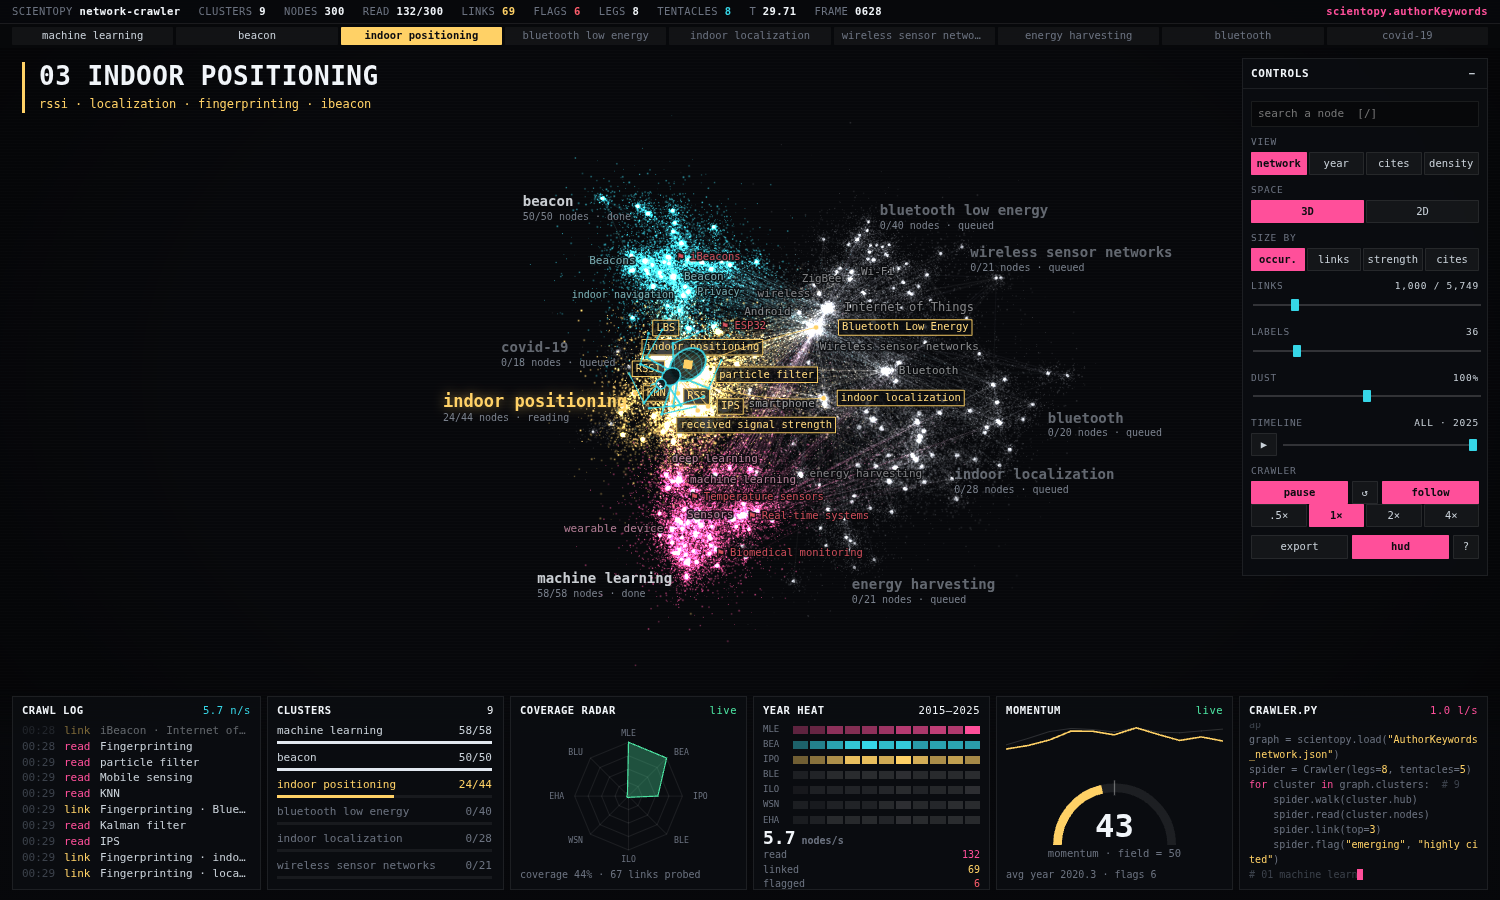
\includegraphics[width=0.95\textwidth]{./figures/network_map.png}
\end{center}

The analysis follows VOSviewer: links are normalized with the association strength, items are clustered by optimizing the VOSviewer quality function (with a resolution parameter), and the map layout uses the VOS mapping technique, in both 3D and 2D. The options of the script are described in Table~\ref{table_network_options}.

\begin{table}[!h]
	\centering
	\caption{Options of scientoPyNetwork.py}
	\label{table_network_options}

	\renewcommand{\arraystretch}{1.4}
	\begin{tabular}{ p{4.6cm} p{12cm}}
	\hline\noalign{\smallskip}
	Option     &  Description                             \\
	\noalign{\smallskip}\hline\noalign{\smallskip}
	\verb|-c|, \verb|--criterion| & Criterion to map, default \verb|authorKeywords| \\
	\verb|-l|, \verb|--length| & Maximum number of items, the top ones by occurrences, default 300 \\
	\verb|--minOccurrences| & Minimum number of documents per item, default 2 \\
	\verb|-s|, \verb|--skipFirst| & Leave out the first N top items \\
	\verb|--exclude| & Items to leave out, separated by \verb|;| \\
	\verb|--synonyms| & Synonym groups or a VOSviewer thesaurus file (see Section~\ref{sec_synonyms}) \\
	\verb|--startYear|, \verb|--endYear| & Year range \\
	\verb|--counting| & \verb|full| or \verb|fractional| counting of co-occurrences \\
	\verb|--minLinkStrength| & Minimum link weight to keep a link \\
	\verb|--resolution| & Clustering resolution, higher gives more and smaller clusters, default 1 \\
	\verb|--minClusterSize| & Smaller clusters are merged into their most connected cluster, default 3 \\
	\verb|--cohesion| & Extra attraction inside clusters in the layout, 0 for the plain VOS mapping, default 0.5 \\
	\verb|-r|, \verb|--previousResults| & Map the documents found by the last \verb|scientoPy.py| run \\
	\verb|--graphTitle| & Title shown in the map \\
	\verb|--noOpen| & Do not open the web browser \\
	\noalign{\smallskip}\hline
	\end{tabular}
\end{table}

The map is a single HTML file that works offline in any recent browser with WebGL2 (Chrome, Edge, Firefox, Safari). It includes:

\begin{itemize}
\item \textbf{Views:} network (clusters), overlay by average publication year or average citations, and density; 3D orbit or flat 2D, with animated transitions.
\item \textbf{Crawler tour:} a spider walks the map one cluster at a time. It reads the items, probes the strongest links, and flags emerging items (recent and growing) and highly cited ones. A dashboard follows it with a crawl log, cluster progress, coverage radar, year heat map, and a momentum gauge.
\item \textbf{Exploration:} search, click an item for its statistics, documents per year, strongest links and most cited documents, timeline playback of the map growth, and the \verb|scientoPy.py| command to analyze it.
\item \textbf{Exports:} PNG and SVG images (dark or light background), videos of the crawl tour, VOSviewer map and network files, GEXF for Gephi, CSV, and JSON.
\end{itemize}

Besides the map, the script writes its data to \verb|results/|: the items, the links, VOSviewer and Gephi files, and \verb|<Criterion>_network_clusters.csv| with the items of every cluster, ready for a table of keywords by cluster.

\subsection{Thematic map}
\label{sec_thematic_map}

The \verb|scientoPyThematicMap.py| script draws the thematic map (strategic diagram) of a criterion. It groups the items that appear together in clusters, the same clusters as \verb|scientoPyNetwork.py| with the same options, and places every cluster (a theme) by two values from Callon's co-word analysis:

\begin{itemize}
\item \textbf{Centrality (relevance degree):} strength of the links between the items of the theme and the items of the other themes. A central theme is tied to the rest of the field.
\item \textbf{Density (development degree):} strength of the links between the items of the theme. A dense theme is well developed.
\end{itemize}

The link strength between two items is the equivalence index:
\begin{equation}
e_{ij} = \frac{c_{ij}^2}{c_i \, c_j}
\label{equation_equivalence}
\end{equation}

where $c_{ij}$ is the number of documents with both items, and $c_i$ and $c_j$ the documents with each one. The centrality of a theme is 10 times the sum of $e_{ij}$ over its links to other themes, and its density is 100 times the sum of $e_{ij}$ over the links inside the theme, divided by its number of items.

\begin{verbatim}
# Thematic map of the author keywords
python3 scientoPyThematicMap.py -c authorKeywords

# Merge synonyms, leave out the search terms and save the plot
python3 scientoPyThematicMap.py -c authorKeywords \
--synonyms "internet of things, iot; bluetooth low energy, ble" \
-s 2 --savePlot "thematic_map.eps"
\end{verbatim}

\begin{center}
	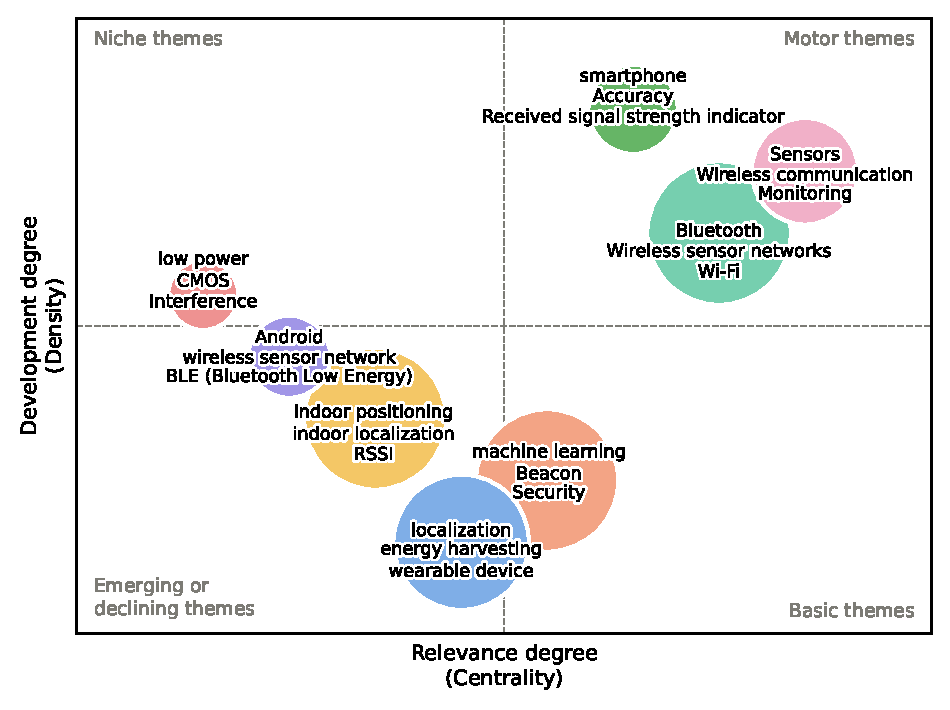
\includegraphics[width=0.75\textwidth]{./figures/graph_thematic_map.eps}
\end{center}

The dashed lines cross at the medians and split the map in four:

\begin{itemize}
\item \textbf{Motor themes} (top right): high centrality and high density. Developed and important for the field.
\item \textbf{Niche themes} (top left): low centrality and high density. Developed, but isolated from the rest.
\item \textbf{Emerging or declining themes} (bottom left): low centrality and low density. Weakly developed and marginal.
\item \textbf{Basic themes} (bottom right): high centrality and low density. Important for the field, but not developed.
\end{itemize}

The bubble area is the number of occurrences of the items of the theme, and each bubble shows its top items. Items that never appear with another item are not part of any theme.

\verb|scientoPyThematicMap.py| takes the options of \verb|scientoPyNetwork.py| that select the items and the clusters (\verb|-c|, \verb|-l|, \verb|--minOccurrences|, \verb|-s|, \verb|--exclude|, \verb|--synonyms|, \verb|--startYear|, \verb|--endYear|, \verb|--counting|, \verb|--minLinkStrength|, \verb|--resolution|, \verb|--minClusterSize|, \verb|-r|, \verb|--graphTitle|), and these ones:

\begin{itemize}
\item \verb|--labels N|: Number of items written on each theme, default 3.
\item \verb|--axes rank| or \verb|--axes value|: \verb|rank| places the themes by their centrality and density ranks, which spreads them evenly (default). \verb|value| places them by the values.
\item \verb|--savePlot "file"|: Save the plot to a file in \verb|graphs/| (png, eps, pdf, svg).
\item \verb|--noPlot|: Only save the table.
\item \verb|--plotWidth N|, \verb|--plotHeight N|: Plot size in inches.
\end{itemize}

The themes, with their centrality, density, quadrant and every item, are saved to \verb|results/<Criterion>_thematic_map.csv|.

\subsection{Most cited documents}
\label{sec_most_cited}

The \verb|topCitedPapers.py| script lists the most cited documents of the dataset:

\begin{verbatim}
# Top 10 most cited documents
python3 topCitedPapers.py

# Top 20, published from 2015 to 2024
python3 topCitedPapers.py -l 20 --startYear 2015 --endYear 2024

# Most cited documents about a topic
python3 scientoPy.py -c authorKeywords -t "indoor positioning" --noPlot
python3 topCitedPapers.py -r
\end{verbatim}

The table is saved to \verb|results/TopCitedPapers.csv| with the citations, the citations per year (citations divided by the years since the document was published), year, title, authors, source, document type, DOI, and EID. The citations are the ones reported by Scopus or WoS when the dataset was downloaded.

\subsection{Output files and directories}

After run some ScientoPy commands or after run all the example commands by executing the script \verb|exampleGenerateGraphs.sh| you will find the following folder and files structure:

\vspace*{0.5cm}
\dirtree{% This % is required
	.1 ScientoPy.
	.2 dataInExample.
	.2 dataPre.
	.3 papersPreprocessed.parquet.
	.3 PreprocessedBrief.csv.
	.2 graphs.
	.3 AuthorKeywords\_network.html.
	.2 Manual.
	.2 results.
	.3 AuthorKeywords.csv.
	.3 AuthorKeywords\_extended.csv.
	.3 AuthorKeywords\_network\_clusters.csv.
	.3 AuthorKeywords\_thematic\_map.csv.
	.3 TopCitedPapers.csv.
	.3 lastAnalysis.parquet.
	.2 export.
	.3 papersPreprocessed.csv.
}

These folders and output files are described bellow:

\begin{itemize}
	\item \textbf{dataInExample: } contains Scopus and WoS example data set for the search criteria "Bluetooth low energy" downloaded in April 2, 2026. This is the input example for preprocess script.

	\item \textbf{dataPre: } output folder for the preprocess results, and input folder for scientoPy script.

	\item \textbf{papersPreprocessed.parquet: } canonical preprocessed corpus (Apache Parquet, Zstd-compressed). Replaces the old \verb|papersPreprocessed.csv| as the input for every other ScientoPy script. Obtain a CSV copy via \verb|exportPapers.py|.
	
	\item \textbf{PreprocessedBrief.csv: } preproceses brief table that shows the preprocess results related to total papers found per data base, the omitted papers, the duplicated papers count per data base, and the total number of papers per paper type (Conference paper, article, review...)
	
	\item \textbf{graphs: } graphs output folder for preprocess and scientoPy scripts

	\item \textbf{AuthorKeywords\_network.html: } interactive network map written by \verb|scientoPyNetwork.py| (self-contained, open it in a web browser).
	
	\item \textbf{Manual: } folder with the pdf manual and example paper with scientoPy commands highlighted used for graph and tables generation. 
	
	\item \textbf{results: } output folder for scientoPy result output files
	
	\item \textbf{AuthorKeywords.csv: } scientoPy output file for the selected criterion (in this case authorKeywords) that shows the top topics or the custom topics with the following columns:
	\begin{itemize}
	\item \textbf{Pos.:} Position in the ranking.
	\item \textbf{[Criterion]:} The topic name for the selected criterion (e.g., AuthorKeywords, Country, Author, etc.).
	\item \textbf{Total:} Total number of documents for this topic.
	\item \textbf{AGR:} Average Growth Rate, the average difference in documents between consecutive years inside the window period. See Eq.~\ref{equation_AGR}.
	\item \textbf{ADY:} Average Documents per Year, the average number of documents published per year inside the window period. See Eq.~\ref{equation_ADY}.
	\item \textbf{PDLY:} Percentage of Documents in Last Years, the percentage of ADY relative to the total number of documents. See Eq.~\ref{equation_PDLY}.
	\item \textbf{hIndex:} h-index for the topic. A topic has h-index $h$ if $h$ of its documents have been cited at least $h$ times.
	\item \textbf{[Year columns]:} Number of documents published in each year within the analysis range.
	\end{itemize}

	\item \textbf{AuthorKeywords\_extended.csv: } scientoPy output file for the selected criterion (in this case authorKeywords) that show the top or custom topics with the documents related to each one.

	\item \textbf{AuthorKeywords\_network\_clusters.csv: } items of every cluster of the network map. \verb|scientoPyNetwork.py| also writes next to it the items (\verb|_network_nodes.csv|), the links (\verb|_network_links.csv|), a JSON file, a GEXF file for Gephi, and the VOSviewer map and network files.

	\item \textbf{AuthorKeywords\_thematic\_map.csv: } themes of the thematic map written by \verb|scientoPyThematicMap.py|, with their centrality, density, quadrant, and items.

	\item \textbf{TopCitedPapers.csv: } most cited documents written by \verb|topCitedPapers.py|.

	\item \textbf{lastAnalysis.parquet: } inside the results folder, this file contains the output papers from the last scientoPy script. It is used as an input for scientoPy when the option \verb|-r| or \verb|--previousResults| is passed. Internal format; not intended for user consumption.

	\item \textbf{export: } on-demand CSV exports produced by \verb|exportPapers.py|. Not created by preprocess or analysis; only populated when the user runs an export.
\end{itemize}

\newpage
\section{ScientoPy graph types}

ScientoPy has 6 different ways to graph the results of \verb|scientoPy.py|, described on Table \ref{table_graph_types}. The network map and the thematic map have their own scripts, described in Sections~\ref{sec_network_map} and~\ref{sec_thematic_map}.

\begin{table}[!h]
	\centering
	\caption{ScientoPy output graphs types}
	\label{table_graph_types}

	\renewcommand{\arraystretch}{1.5}
	\begin{tabular}{ p{4cm} p{3cm} p{10cm}}
	\hline\noalign{\smallskip}
	Graph type     &  Argument & Description                             \\
	\noalign{\smallskip}\hline\noalign{\smallskip}                                                                         
	Time line      & \verb|-g time_line| & Graphs the number of documents of each topic vs the publication year \\
	Horizontal bars  & \verb|-g bar| & Graphs the total number of documents of each topic in horizontal bars \\
	Horizontal bars trends  & \verb|-g bar_trends| & Graphs the total number of documents of each topic in horizontal bars, with the percentage of document published in the last years \\
	Evolution     & \verb|-g evolution| & Graphs two plots: on the left, the accumulative number of documents (logarithmic scale) vs. the publication year, where the beginning of each line shows when the topic research started and the final value represents the total number of documents; on the right, a scatter plot of the Average Growth Rate (AGR) on the Y-axis vs. the Percentage of Documents in Last Years (PDLY) on the X-axis, allowing comparison of absolute and relative growth for each topic \\
	Word cloud     & \verb|-g word_cloud| & Generate a word cloud based on the topic total number of publications \\
	World map     & \verb|-g world_map| & Shades every country by its number of documents, only for the \verb|country| criterion \\
	\noalign{\smallskip}\hline
	\end{tabular}
\end{table}

Below are showed some examples of these graphs types, with the command used.

\subsection{Time line graph}
Command: 
\begin{verbatim}
python3 scientoPy.py -c authorKeywords --startYear 2015 --endYear 2025 -g time_line
\end{verbatim}

\begin{center}
	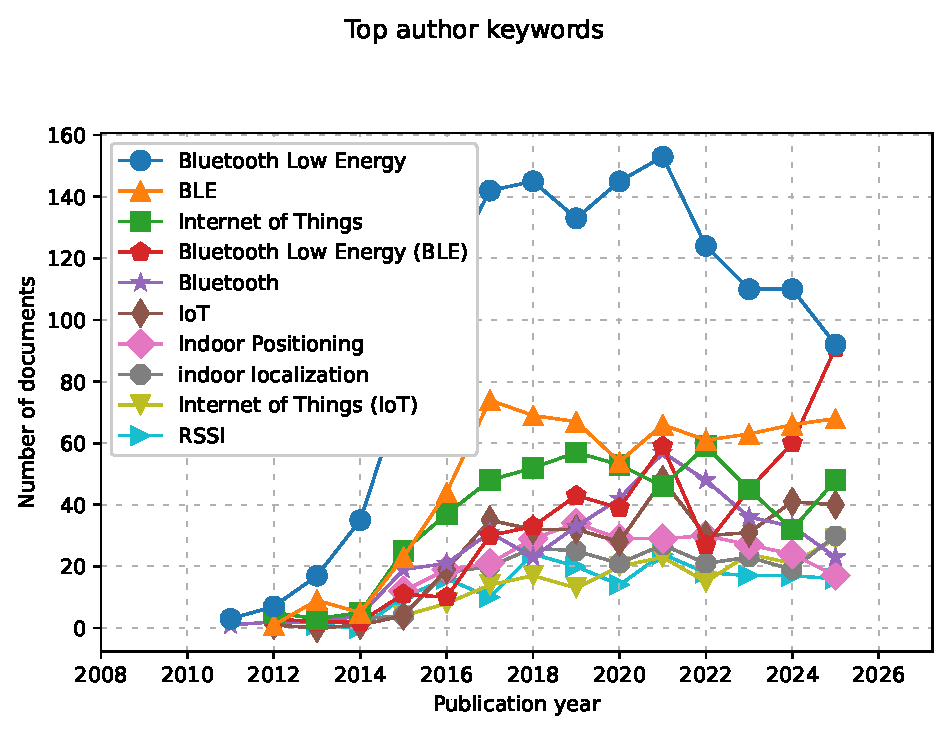
\includegraphics[width=0.75\textwidth]{./figures/graph_time_line.eps}
\end{center}

\subsection{Horizontal bars graph}
Command: 
\begin{verbatim}
python3 scientoPy.py -c authorKeywords --startYear 2015 --endYear 2025 -g bar
\end{verbatim}

\begin{center}
	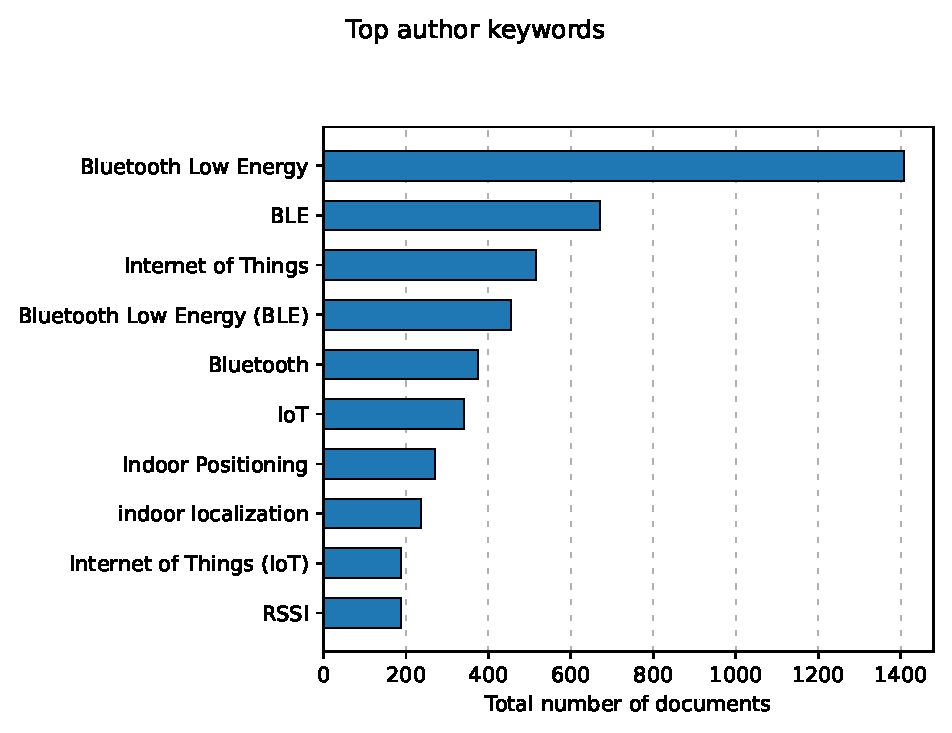
\includegraphics[width=0.75\textwidth]{./figures/graph_bar.eps}
\end{center}

\subsection{Horizontal bars trends}
Command: 
\begin{verbatim}
python3 scientoPy.py -c authorKeywords --startYear 2015 --endYear 2025 -g bar_trends
\end{verbatim}

\begin{center}
	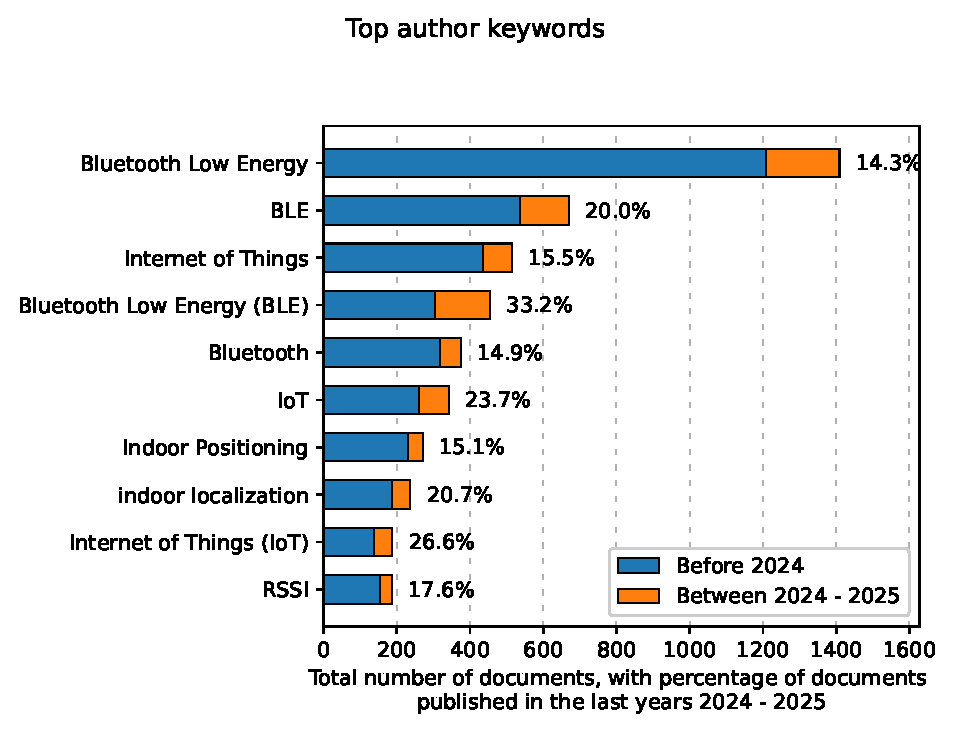
\includegraphics[width=0.75\textwidth]{./figures/graph_bar_trends.eps}
\end{center}

\subsection{Evolution graph}
Command:
\begin{verbatim}
python3 scientoPy.py -c authorKeywords --startYear 2015 --endYear 2025 -g evolution
\end{verbatim}

\begin{center}
	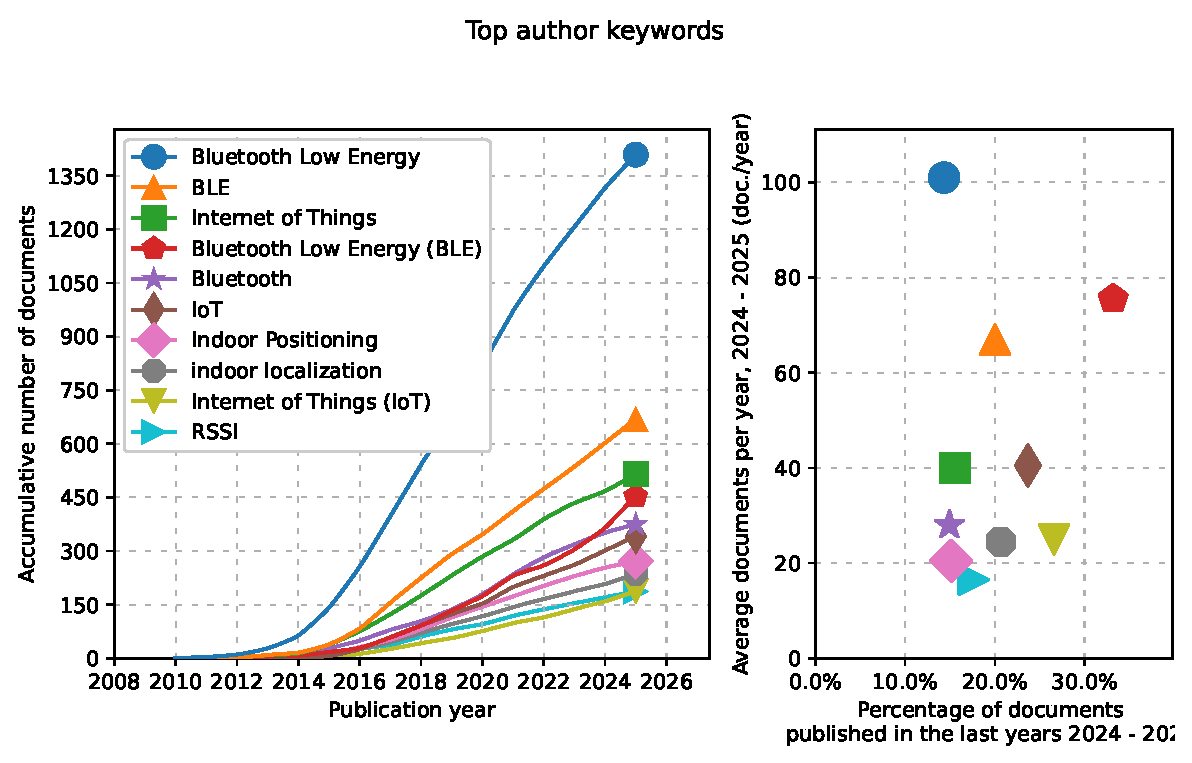
\includegraphics[width=0.75\textwidth]{./figures/graph_evolution.eps}
\end{center}

The evolution graph shows two panels:
\begin{itemize}
\item \textbf{Left panel (Accumulative documents):} The X-axis represents the publication year and the Y-axis the accumulative number of documents (in logarithmic scale). The beginning of each line indicates when the topic research started, and the final value of each line represents the total number of documents published for that topic.
\item \textbf{Right panel (AGR vs. PDLY):} The Y-axis represents the AGR (Average Growth Rate) for the specified window period, and the X-axis represents the PDLY (Percentage of Documents in Last Years). Topics with higher AGR have the highest absolute growth, and topics with higher PDLY have the highest relative growth. This allows identifying which topics are trending (high AGR and high PDLY) versus which are established but declining.
\end{itemize}


\subsection{Word cloud graph}
Command: 
\begin{verbatim}
python3 scientoPy.py -c authorKeywords --startYear 2015 --endYear 2025 -l 500 -g word_cloud
\end{verbatim}

\begin{center}
	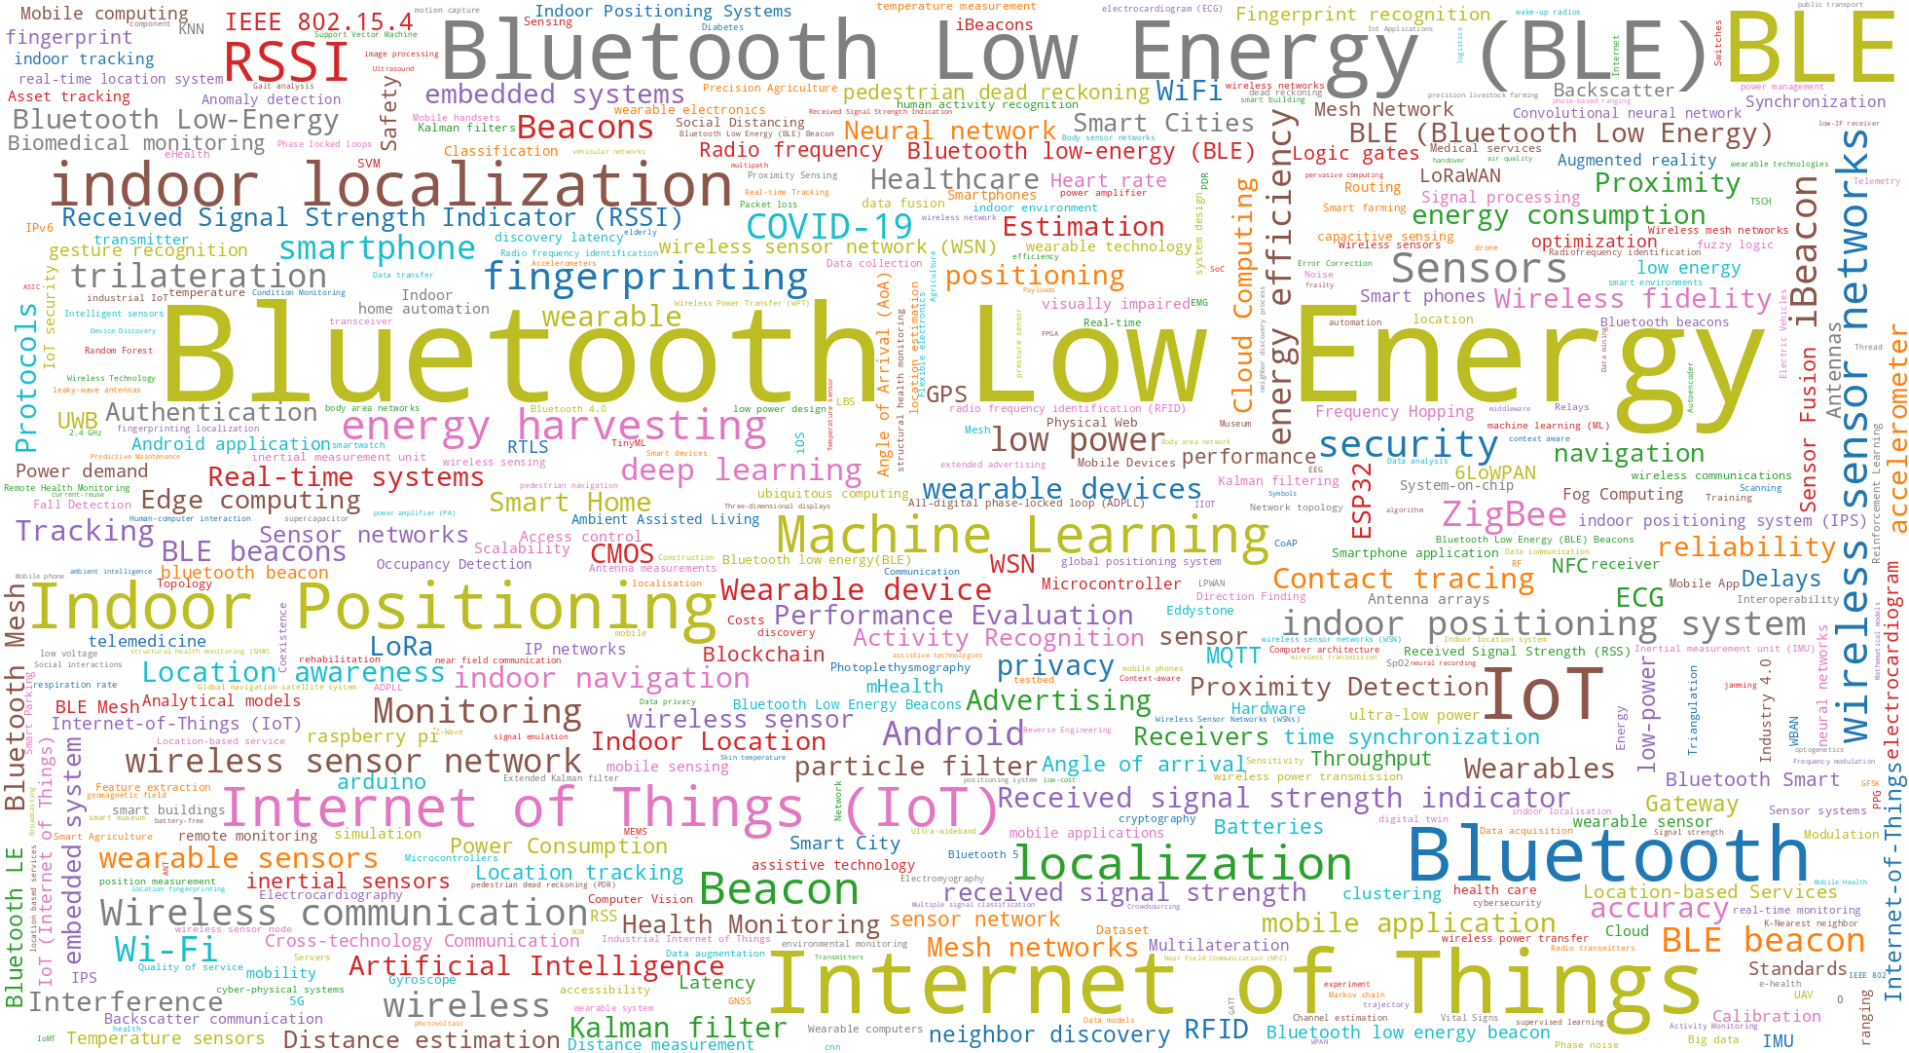
\includegraphics[width=0.9\textwidth]{./figures/graph_word_cloud.png}
\end{center}

\subsection{World map graph}
\label{sec_graph_world_map}
Command:
\begin{verbatim}
python3 scientoPy.py -c country --startYear 2015 --endYear 2025 -g world_map
\end{verbatim}

\begin{center}
	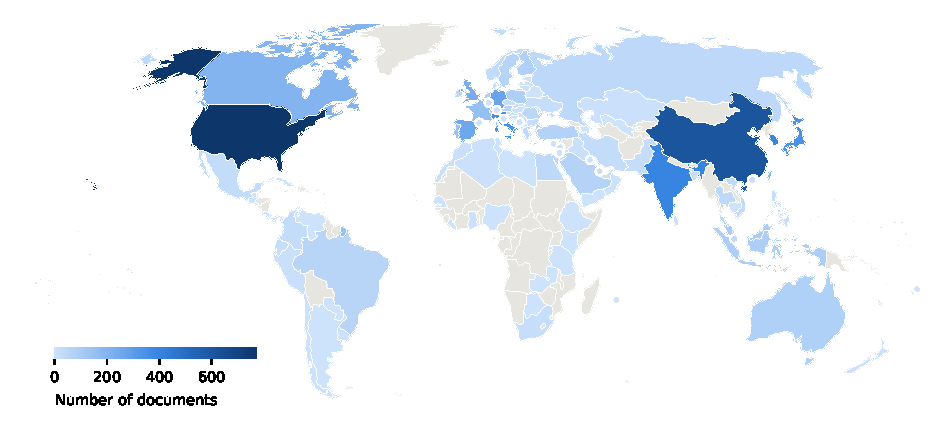
\includegraphics[width=0.9\textwidth]{./figures/graph_world_map.eps}
\end{center}


\newpage
\section{BibTeX generation}

ScientoPy can automatically generate a BibTeX bibliography file from a LaTeX document. This feature matches \verb|\cite{}| keys used in the LaTeX file against the preprocessed dataset, and produces a \verb|.bib| file with the corresponding entries.

\subsection{How it works}

The \verb|generateBibtex.py| script performs the following steps:

\begin{enumerate}
\item Reads the input LaTeX file and extracts all \verb|\cite{key}| references from the document body (between \verb|\begin{document}| and \verb|\begin{thebibliography}|).
\item Loads the preprocessed dataset (\verb|dataPre/papersPreprocessed.parquet|).
\item Matches each citation key against the EID field of the papers in the dataset.
\item Generates BibTeX entries for matched papers:
\begin{itemize}
\item \verb|@Article{}| for journals, reviews, and articles in press.
\item \verb|@Inproceedings{}| for conference papers and proceedings papers.
\end{itemize}
\item Handles author name formatting, converting Scopus and WoS formats into BibTeX's \verb|and|-separated format.
\item Escapes LaTeX special characters (\verb|&|, \verb|_|) in titles and other fields.
\item Saves the output file next to the input file, with the suffix \verb|_bibliography.bib|. For example, \verb|myPaper.tex| produces \verb|myPaper_bibliography.bib|.
\end{enumerate}

\subsection{Usage}

\textbf{Prerequisites:} The preprocessing step must be completed first, so that the file \verb|dataPre/papersPreprocessed.parquet| exists.

\subsubsection{Using the cite keys}

In your LaTeX document, use the paper's EID as the cite key. The EID can be found in the extended results file (\verb|results/*_extended.csv|) under the \textbf{EID} column. For example:

\begin{verbatim}
\cite{WOS:000363238300013}
\cite{WOS:000371717205060, WOS:000380412500076}
\end{verbatim}

\subsubsection{Running from the command line}

To generate the BibTeX file, run:

\begin{verbatim}
python3 generateBibtex.py latexExample/article_example.tex
\end{verbatim}

This will create the file \verb|latexExample/article_example_bibliography.bib|.

\subsubsection{Compiling the LaTeX document}

In your LaTeX document, reference the generated bibliography:

\begin{verbatim}
\bibliographystyle{unsrt}
\bibliography{article_example_bibliography}
\end{verbatim}

Then compile with the standard LaTeX/BibTeX cycle:

\begin{verbatim}
pdflatex article_example
bibtex article_example
pdflatex article_example
pdflatex article_example
\end{verbatim}

A Makefile is provided in the \verb|latexExample/| folder that automates this process. Run \verb|make| inside that folder to generate the bibliography and compile the PDF in one step.

\subsubsection{Using the GUI}

In the ScientoPy graphical interface, click the \textbf{Generate BibTeX} button on the Analysis tab. This will open a file dialog to select your LaTeX file, generate the bibliography, and open the resulting \verb|.bib| file.

\end{document}
